\subsection{Recap: How to Implement Features?}
\begin{frame}{\myframetitle}
	\begin{mycolumns}
		\myexampletight{Given a feature model for graphs \ldots}{
			\centering\featureDiagramGraphs
			%\featureDiagramLegend
		}
		\myexample{\ldots\ we can derive a valid configuration}{
			\small
			\leftmiddleandright{
				$\{G\}$\\
				$\{G,C\}$\\
				$\{G,D\}$\\
				$\{G,C,D\}$\\
			}{
				$\{G,W\}$\\
				$\{G,C,W\}$\\
				$\{G,D,W\}$\\
				$\{G,C,D,W\}$\\
			}{
				$\{G,W,S\}$\\
				$\{G,C,W,S\}$\\
				$\{G,D,W,S\}$\\
				$\{G,C,D,W,S\}$\\
			}
		}
	\mynextcolumn
		\vspace{-10mm}
		\myexampletight{How to Generate Products Automatically?}{
			\centering\foreach \page in {2,12,4,14,6,16,8,18,10,20,42,44}{\includegraphics[width=.23\linewidth,page=\page]{graphs} }
		}
		\mynote{Goals}{
			\begin{itemize}
				\item Descriptive specification of a product (i.e., a configuration, a selection of features)
				\item Automated generation of a product with compile-time variability
			\end{itemize}			
		}
	\end{mycolumns}
\end{frame}

\begin{frame}{Recap: Features with Build Systems}
	\begin{mycolumns}[widths={40,60},animation=none]
		\myexampletight{}{
			\centering
			\pic[width=.65\linewidth]{pignap-features}
		}
	\mynextcolumn
		\mydefinition{Conditional Compilation with Build Systems}{
			\begin{itemize}
				\item Exploit the expressiveness of a build system's configuration language
				\item In- and exclude individual files or entire directories based on feature selection
			\end{itemize}
		}
		\uncover<2->{\mynote{Major Challenges}{
			\begin{itemize}
				\item Build scripts may become complex, there is no limit to what can be done (e.g., you can run arbitrary shell commands on files)\\
					$\Rightarrow$ \emph{Hard to understand and analyze}
				\item No simple in- and exclusion of individual lines or chunks of code\\
					$\Rightarrow$ High-level use \emph{only}!
			\end{itemize}
		}}
	\end{mycolumns}
\end{frame}

\begin{frame}{Recap: Features with Preprocessors}
	\begin{mycolumns}[widths={40,60},animation=none]
		\myexampletight{}{
			\centering
			\pic[width=\linewidth,page=1,trim=15 20 185 40,clip]{preprocessor-wilderness}
		}
	\mynextcolumn
		\mydefinition{Conditional Compilation with Preprocessors}{
			\begin{itemize}
				\item Use conditional compilation facilities provided by preprocessors 
				\item Annotate and potentially remove code fragments, depending on feature selection
			\end{itemize}
		}
		\uncover<2->{\mynote{Major Challenges}{
			\begin{itemize}
				\item May \emph{obfuscate} source code and severely impact its readability
				\item Hard to analyze and process for existing IDEs
				\item Often used in an ad-hoc or \emph{undisciplined} fashion
				\item Prone to subtle syntax, type, or runtime errors which are hard to detect
				\item \emph{Scattering} and \emph{tangling}\\
					$\Rightarrow$ Separation of concerns?
			\end{itemize}
		}}
	\end{mycolumns}
\end{frame}

\begin{frame}{Modularity}
	\begin{mycolumns}[widths={50,50},animation=none]
		\mydefinition{Modularization}{
			Consistent application of \emph{information hiding} and \emph{data encapsulation}:
			\begin{itemize}
				\item Strong logical connection between the inner parts of a module (high cohesion)
				\item Precisely defined, minimal interfaces (low coupling)
			\end{itemize}						
		}
	\mynextcolumn
		\mydefinition{Coupling and Cohesion}{
			\begin{itemize}
				\item Cohesion: Measure of how well the parts of a module work together (intra-module communication).
				\item Coupling: Measure of the complexity of inter-module communication (through interfaces).
			\end{itemize}
		}
	\end{mycolumns}
	\begin{mycolumns}[widths={50,50},animation=none]
		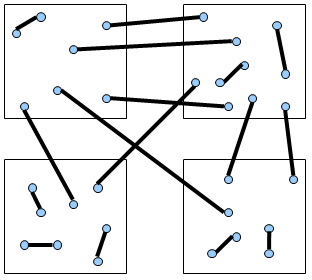
\includegraphics[width=\textwidth]{cohesion_coupling_1}
	\mynextcolumn
		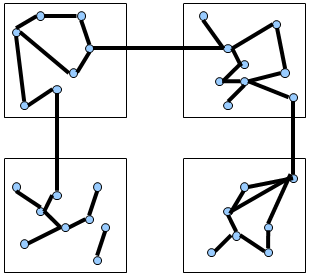
\includegraphics[width=\textwidth]{cohesion_coupling_2}
	\end{mycolumns}
\end{frame}

\begin{frame}{Why Modularity?}
	\begin{mycolumns}[widths={50,50},animation=none]
		\mynote{Traditional Reasons}{			
			\begin{itemize}
				\item Modules can be developed independently of each other (collaborative work)
				\item Easier to maintain because changes can be made locally
				\item Data encapsulation promotes stability and reliability
				\item Software is easier to understand:
				\item Hiding complexity behind interfaces
				\item Modular decomposition = divide and conquer
			\end{itemize}						
		}
	\mynextcolumn
		\mynote{Modularization and Software Product Lines}{
			\begin{itemize}
				\item Reuse: Parts of the software can be {\em reused} 
				\item Alternatives: Modules can be {\em exchanged by alternative implementations}
				\item Variability: Modules can be {\em reassembled in a new context} (e.g., in other projects)
			\end{itemize}
		}
		\myexampletight{}{
			
\includegraphics[width=\linewidth,page=18,trim=5 5 5 5,clip]{lego} 
		}
	\end{mycolumns}	
\end{frame}

\begin{frame}{Components}
	\begin{mycolumns}[widths={50,50},animation=none]
		\mydefinition{Component \mysource{\szyperski}}{			
			A software component is a unit of composition with contractually specified interfaces and explicit context dependencies only. 
			A software component can be deployed independently and is subject to composition by third parties.
		}
		\mynote{}{			
			\begin{itemize}
				\item Provides its functionality through an interface (provided interface)
				\item Declares functional dependencies to other components (required interface)
				\item Declares deployment dependencies such as container or middleware (e.g., JavaEE, COBRA, COM+/DCOM, OSGi, etc.)
			\end{itemize}
		}
		\myexampletight{}{
			\centering
			\pic[width=.5\linewidth]{component_uml.png}
		}	
	\mynextcolumn
		\mynote{Composition and Reuse}{
			Components
			\begin{itemize}
				\item are composed with other components to form software systems,
				\item are supposed to be re-usable in other software systems,
				\item may stem from third-party vendors (make-or-by-decisions, markets for components).
			\end{itemize}			
		}
		\myexampletight{}{
			\centering
			\pic[width=.8\linewidth]{component_diagram_uml.png}
		}	
	\end{mycolumns}	
\end{frame}

\begin{frame}{Components vs. Objects/Classes}
	\begin{mycolumns}[widths={40,60},animation=none]
		\mynote{Commonalities}{			
			Lots of similar priniples, particularly 
			\begin{itemize}
				\item encapsulation and information hiding,  
				\item accessibility through public interfaces,
				\item (de-)composition and nested objects/components,
				\item etc.				
			\end{itemize}
		}
	\mynextcolumn
		\mynote{Differences}{
			\begin{itemize}
				\item Objects are smaller than components by focusing on detailed implementation problems (components aim at abstracting from implementation details).
				\item Object are less cohesive and stronger coupled than components due to (deliberately) delegating lots of responsibilities to other objects, while components aim at maximizing cohesion and minimizing coupling.
				\item Objects/classes are reused through inheritance and polymorphism, while components are reused by being integrated into a component architecture.		
			\end{itemize}			
		}
	\end{mycolumns}	
\end{frame}

\begin{frame}[fragile]{Example: A Color Component}
	\begin{mycolumns}[columns=2,widths={50,50}]
{\tiny
\begin{codetight}{}
package components.color;

~// public interface~
public class ColorComponent {
	public Color createColor(int r, int g, int b) { /* ... /* }
	public void printColor(Color color) { /* ... /* }
	public void mapColor(Object o, Color c) { /* ... /* }
	public Color getColor(Object o) { /* ... /* }
	
	// just one component instance
	public static ColorComponent getInstance() { return instance; }
	private static ColorComponent instance = new ColorComponent();
	private ColorComponent() { super(); }
}
public interface Color { /* ... /* }

// hidden implementation
class ColorImpl implements Color { /* ... /* }
class ColorPrinter { /* ... /* }
class ColorMapping { /* ... /* }
\end{codetight}
}
		\mynextcolumn
			\myexample{A Reusable Component}{
				\begin{itemize}
					\item Assume that storing and printing colors is non-trivial (e.g., in our graph library). 
					\item Implement color management as a reusable component, using Java's visibility mechanism to enforce encapsulation.						
				\end{itemize}
			}
	\end{mycolumns}
\end{frame}

\begin{frame}[fragile]{Example: A Color Component}
	\begin{mycolumns}[columns=2,widths={50,50}]
{\tiny
\begin{codetight}{}
public class Node {
	int id;

	public Node(int id) {
		this.id = id;
	}

	public Node(int id, Color c) {
		this(id);
		ColorComponent.getInstance().mapColor(this, c);
	}

	public void print() {
		if (Config.COLORED) {
			Color c = ColorComponent.getInstance().getColor(this);
			ColorComponent.getInstance().printColor(c);
		}
		System.out.print(id);
	}
}
\end{codetight}
\begin{codetight}{}
public class Graph {
	private List<Node> nodes = new ArrayList<Node>();

	public Node add() {
		Node n = null;
		if (Config.COLORED) {
			Color c = ColorComponent.getInstance().createColor(255, 255, 255);
			n = new Node(nodes.size(), c);
		} else {
			n = new Node(nodes.size());
		}
		nodes.add(n);
		return n;
	}
	~// ...~
}
\end{codetight}
}
		\mynextcolumn
			\mynote{Reuse + Glue Code}{
				\begin{itemize}
					\item We can reuse the Color Component when implementing the color feature for the graph library (but also for other applications). 
					\item However, we need to write custom code to ``connect'' our implementation with the component.\\
						$\Rightarrow$ \emph{Glue Code}
				\end{itemize}
			}
	\end{mycolumns}
\end{frame}


\begin{frame}{Component-Based Implementation of Software Product Lines}
	\begin{mycolumns}[widths={40,60},animation=none]
		\mydefinition{General Idea}{					
			\begin{itemize}
				\item Every feature is implemented by a dedicated component.
				\item Feature selection determines which components shall be integrated to form an application.				
			\end{itemize}
		}
		\myexample{Vision}{
			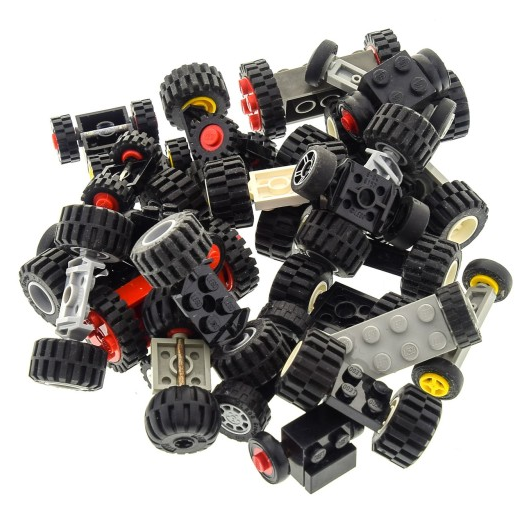
\includegraphics[width=.38\linewidth,height=1.75cm]{lego_components} 
				\vspace*{\fill}
					$\Longrightarrow$ 
				\vspace*{\fill}	
			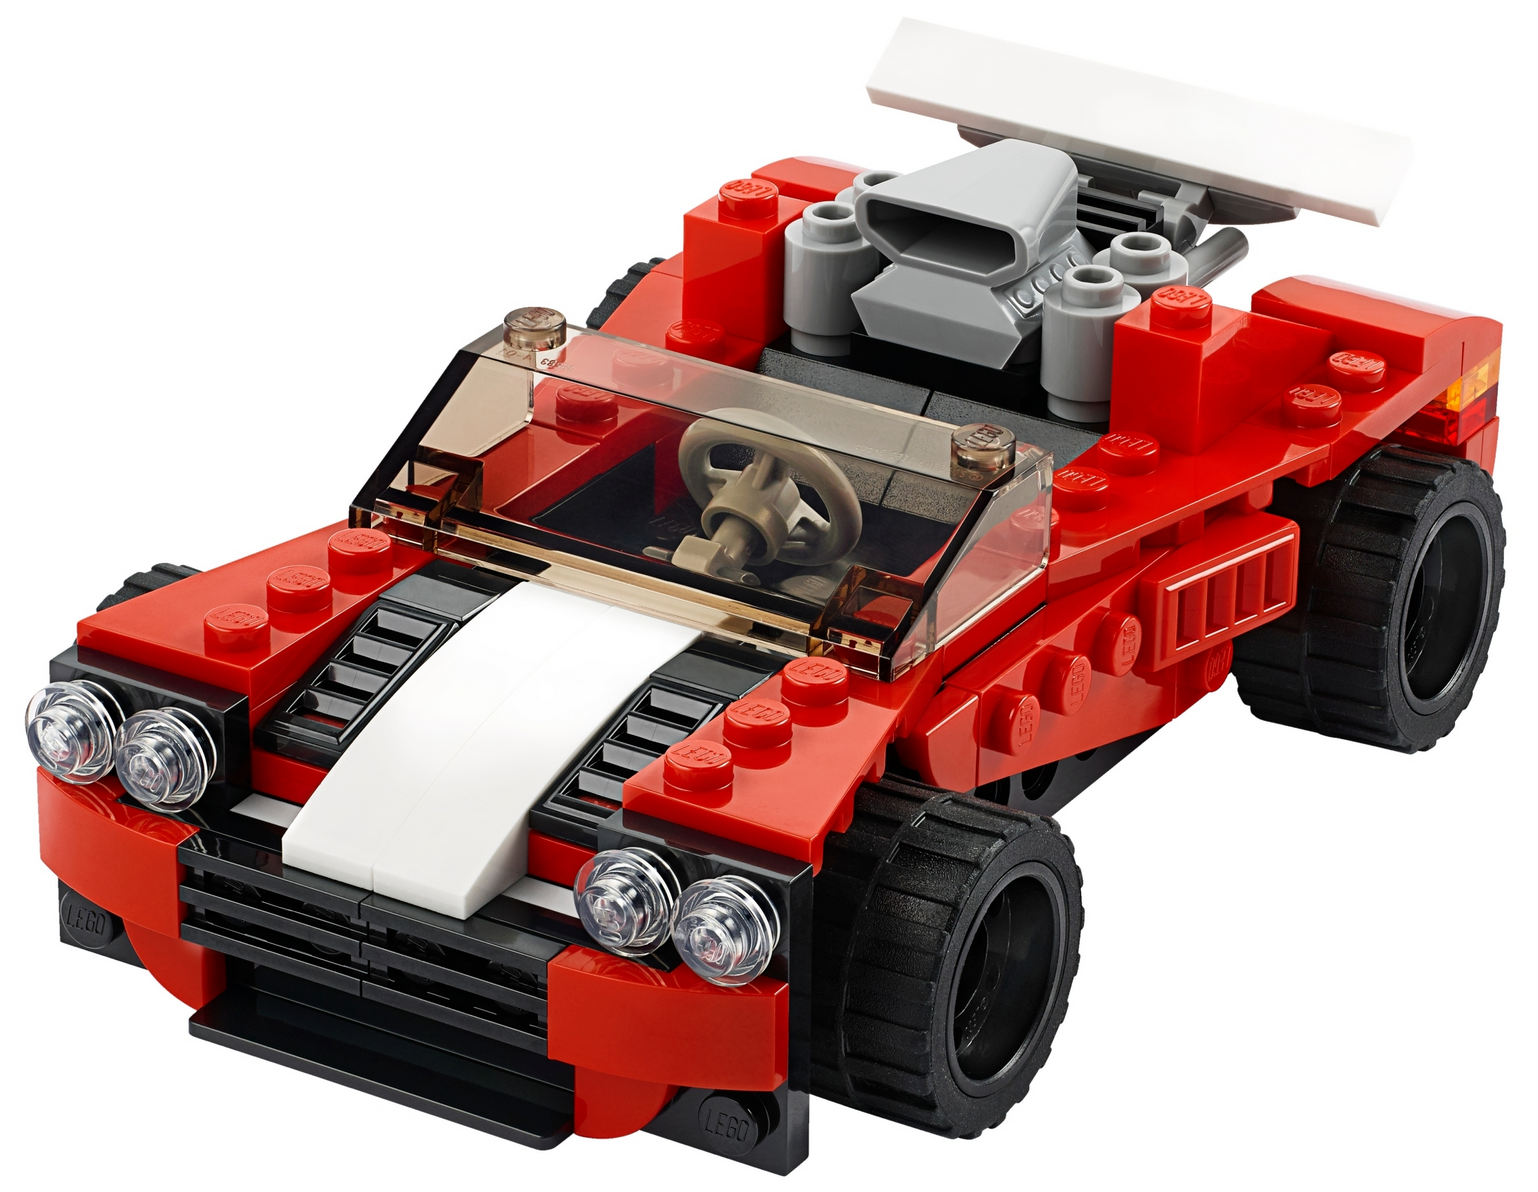
\includegraphics[width=.47\linewidth,height=1.75cm]{lego_product}
		}
	\mynextcolumn
		\myexample{Reality}{
			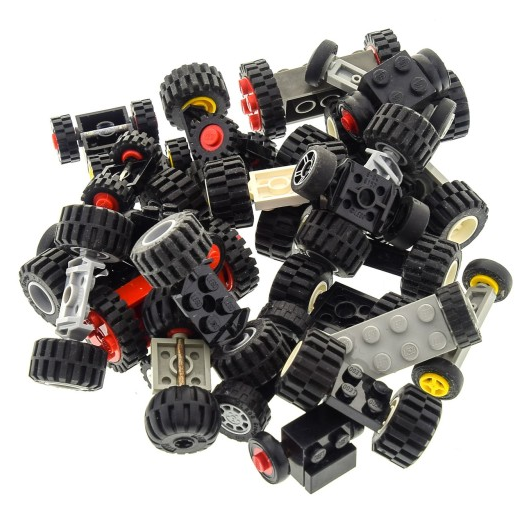
\includegraphics[width=.27\linewidth,height=1.75cm]{lego_components} 
				\vspace*{\fill}
					$+$ 
				\vspace*{\fill}	
			
\includegraphics[width=.27\linewidth,height=1.75cm]{lego_glue}
				\vspace*{\fill}
					$=$ 
				\vspace*{\fill}	
			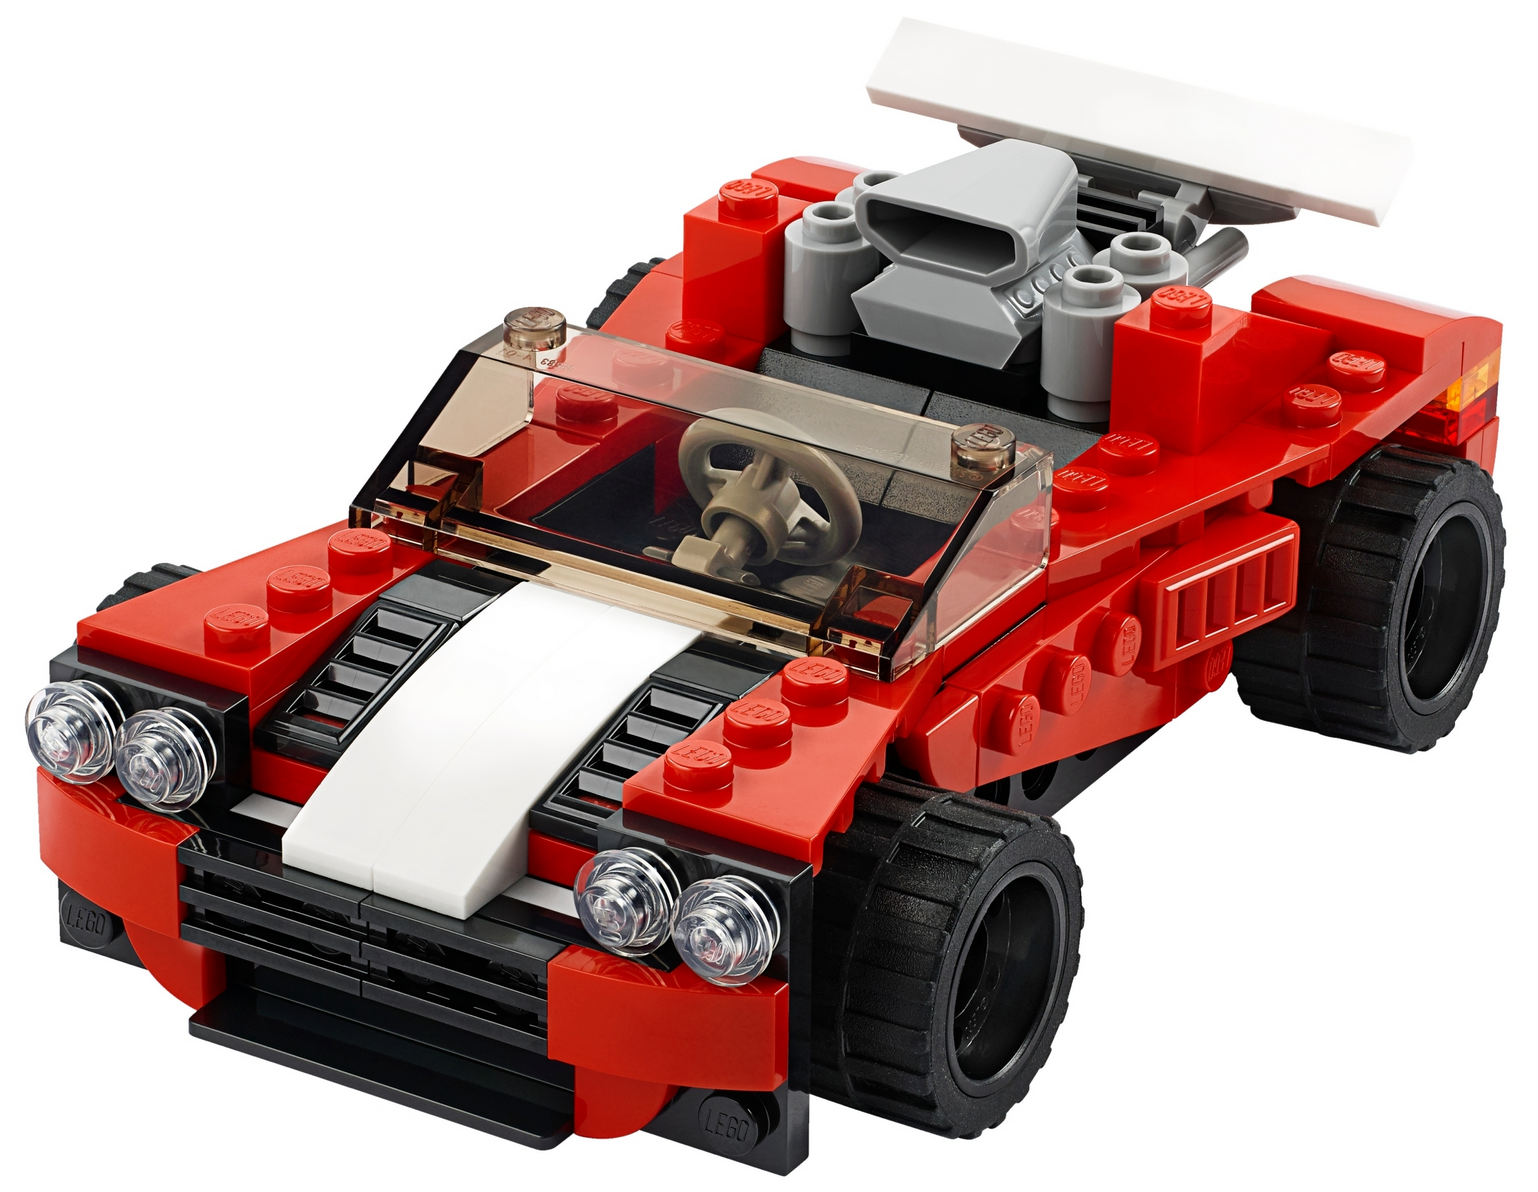
\includegraphics[width=.35\linewidth,height=1.75cm]{lego_product}
		}			
		\mynote{Glue Code and Customization}{
			\begin{itemize}
				\item Developers must connect components through glue code (exception: If components are only exchanged against alternative components are exchanged, no glue code is required)
				\item Components may contain run-time variability (e.g., color manager in our example may be parameterized by color model (RGB, CMYK, ...))
			\end{itemize}
		}
	\end{mycolumns}	
\end{frame}

\begin{frame}{The Library Scaling Problem}
TODO
\end{frame}

\subsection{Recap: UML Component Diagram}
\subsection{Vision: Component Markets}
\subsection{The Library Scaling Problem}
\subsection{Components in Java}
\subsection{Components for Features}
\subsection{Discussion}

